% THIS IS SIGPROC-SP.TEX - VERSION 3.1
% WORKS WITH V3.2SP OF ACM_PROC_ARTICLE-SP.CLS
% APRIL 2009
%
% It is an example file showing how to use the 'acm_proc_article-sp.cls' V3.2SP
% LaTeX2e document class file for Conference Proceedings submissions.
% ----------------------------------------------------------------------------------------------------------------
% This .tex file (and associated .cls V3.2SP) *DOES NOT* produce:
%       1) The Permission Statement
%       2) The Conference (location) Info information
%       3) The Copyright Line with ACM data
%       4) Page numbering
% ---------------------------------------------------------------------------------------------------------------
% It is an example which *does* use the .bib file (from which the .bbl file
% is produced).
% REMEMBER HOWEVER: After having produced the .bbl file,
% and prior to final submission,
% you need to 'insert'  your .bbl file into your source .tex file so as to provide
% ONE 'self-contained' source file.
%
% Questions regarding SIGS should be sent to
% Adrienne Griscti ---> griscti@acm.org
%
% Questions/suggestions regarding the guidelines, .tex and .cls files, etc. to
% Gerald Murray ---> murray@hq.acm.org
%
% For tracking purposes - this is V3.1SP - APRIL 2009

\documentclass{acm_proc_article-sp}

\usepackage[ngerman]{babel}
\usepackage[utf8]{inputenc}
\usepackage{tikz}
\usepackage{float}


\begin{document}

%\title{Complex Network Analysis mit R}
%\subtitle{Kategorien bei Artikeln eines wissenschaftlichen Fachsgebiets in der Wikipedia}
\title{Kategorien bei Artikeln eines wissenschaftlichen Fachsgebiets in der Wikipedia}

\numberofauthors{1} 
\author{
% 1st. author
\alignauthor
	First Author\\
	\affaddr{Universität}\\
	\email{peterr@github.com}
}

\maketitle
\begin{abstract}
	Das ist mein Abstract.
\end{abstract}

\section{Einführung}
In der Wikipedia werden den Artikel Kategorien zugeordnet. Ein Artikel kann in beliebig viele Kategorien gelistet werden. Der Aufbau der Kategorien ist hierachisch. 

- What is your research question or your goal in your class project?
\subsection{Fragestellung}
- How can you answer your question or realize your goal?
Bildet die Kategorisierung der Artikel in der Wikipedia, die Forschungsgebiete der Wissenschaft ab? Dass heißt bilden sich Gruppen von Kategorien, die wissenschaftlich nahe verwandt sind?

\section{Datensatz}
Der Datensatz für die Analyse der Kategorien von wissenschaftlichen Fachgebieten wurde über die API der englischen Wikipedia gewonnen. Es wurde die Kategorie \textbf{machine Learning} als beispielhaftes Themengebiet ausgewählt, um die Analyse durchzuführen. Bei unserer Analyse wurde nur die Artikel berücksichtigt, die direkt unter der Kategorie als Seiten aufgelistet werden.
- How can you answer your question or realize your goal?
Bildet die Kategorisierung der Artikel in der Wikipedia, die Forschungsgebiete der Wissenschaft ab? Dass heißt bilden sich Gruppen von Kategorien, die wissenschaftlich nahe verwandt sind?
\subsection{Aufbau des Netzwerks}
Die Kategorien der Artikel bilden in unserem Netzwerk bilden die Knoten und haben außer dem Namen der Kategorie keine weiteren Eigenschaften. Die Kanten zwischen den Kategorien beschreiben die Bezeihung, dass beide Kategorien zusammen einem Artikel zugeordnet wurden. 
\begin{figure}[H]
\centering
\begin{tikzpicture}[scale=2]
	\tikzstyle{every node}=[sloped,draw,shape=rectangle];
\node            (a) at (0,0)  {Kategorie A};
\node[draw=none] (art1) at (1,-0.2) {in Artikel 1};
\node[draw=none] (art2) at (1,0.45) {in Artikel 2};
\node[draw=none] (art3) at (0.05,-0.5) {in Artikel 1};
\node[draw=none] (art4) at (1.95,-0.5) {in Artikel 2};
\node            (b) at (2,0)  {Kategorie B };
\node            (c) at (1,-1) {Kategorie C };
\draw[-, bend right] (a) edge (b); 
\draw[-, bend left] (a) edge (b);
\draw[-] (a) edge (c);
\draw[-] (b) edge (c);
\end{tikzpicture}
\caption{Struktur des Netzwerkes}
\end{figure}
Die Kanten sind ungerichtet, da beide Kategorien in einem Artikel immer zusammen verwendet werden. Zwischen zweiKnoten können keine, eine oder mehr Kanten existieren. Mehr als eine Kanten zwischen zwei Knoten, existieren nur, wenn die beiden Kategorien in mehreren Artikel zusammen verwendet werden.
\section{Eigenschaften des Netzwerkes}
Das hier vorliegende Netzwerk, dass die Kategorisierung von Artikel der Kategorie maschinelles Lernen darstellt, existieren alle Kanten nur einmal. Das heißt jede der Kombinationen von Kategorien wurde nur einmal vergeben.
Für die weitere Analyse wurde die Kategorie Machine Learning aus dem Graph entfernt, da diese in jedem Artikel auftritt. Dieser Umstand ist dem Verfahren zum Erzeugen des Netzwerkes geschuldet.
\begin{figure}[H]
\centering
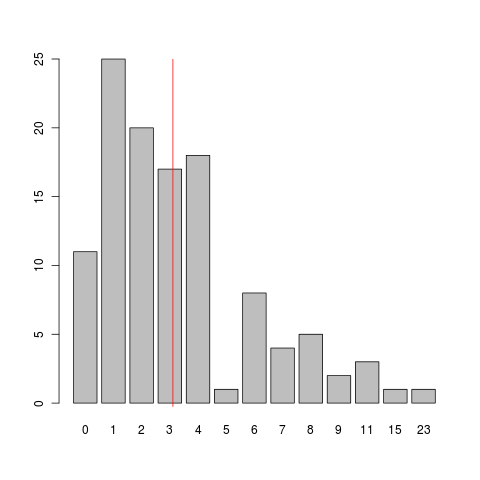
\includegraphics[scale=0.35]{../visualization/degree_hist.png}
\caption{Gradverteilung des Netzwerks}
\end{figure}
degree\\
Die durschnittliche Gradanzahl der Knoten beträgt $3.4$ und der maximale Grad eines Knoten ist $23$. Der Knoten mit dem maximalen Grad ist die Kategorie \textbf{Data Mining}. Außerdem haben $11$ Knoten keine Kanten, sie sind also von den anderen Kategorien isoliert.
dichte\\
Die Dichte des Netzwerkes beträgt $2.9\%$. Es handelt sich also um ein Netzwerk, dass angesichts der maximal möglichen Kanten, nur sehr dünn verbunden ist.
transitivity\\
Der globale Clusterkoeffizient des Netzwerkes hat einen Wert von $53\%$. Dasbedeutet eine Kategorie hat mit einer $50$-prozentigen Wahrscheinlichkeit eine Verbindung zu einer anderen Kategorie.
\subsection{Centralization}
\subsubsection{degree}
\subsubsection{betweenness}
\subsubsection{closeness}
\subsection{Cluster}
\subsection{Communities}
\section{Analyse}
\begin{figure}
\centering
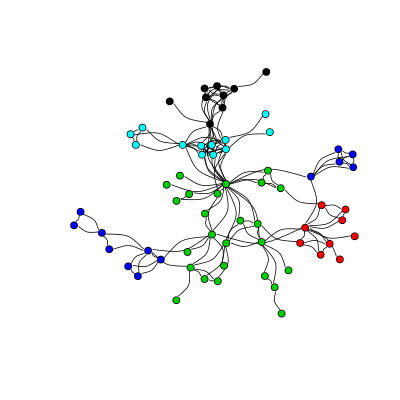
\includegraphics[scale=0.5]{../visualization/ml_community_graph.png}
\caption{Netzwerk in dem Gebiet maschinelles Lernen}
\end{figure}
\section{Ergebnisse}
\section{Related Work}
\section{Zusammenfassung und Ausblick}
\cite{*}
\bibliographystyle{abbrv}
\bibliography{report}

\end{document}  % This is where a 'short' article might terminate
